\ifdefined\ishandout
\documentclass[handout, 10pt]{beamer}
\else
\documentclass[10pt]{beamer}
\fi

%\usepackage[frenchb]{babel}
\usepackage[T1]{fontenc}
%\usepackage[utf8]{inputenc}
\usepackage{hyperref}
\usepackage{multirow}
\usepackage{listings}
\usepackage{fancyvrb}
\usepackage{tikz}
\usepackage{framed}
\usepackage{xmpmulti}
\usepackage{algorithm}
\usepackage{algorithmicx}
\usepackage{algpseudocode}
\usepackage{xcolor}
\usepackage{booktabs}
\usepackage{color, colortbl}
\ifdefined\ishandout
\usepackage{handoutWithNotes}
\fi
\usepackage{slashbox}
\usepackage{amsmath}
\usepackage{bm}
\usepackage{hhline}
\usepackage{pgfplots}
\usepackage{caption}
\graphicspath{{../old/course-utrecht/fig/}{../old/course-utrecht/fig/L1/}{../old/course-utrecht/fig/L2/}{../old/course-utrecht/fig/L3/}} %Setting the graphicspath

\def\UrlBreaks{\do\/\do-}

\usetikzlibrary{shapes.geometric}
\usetikzlibrary{positioning}
\usetikzlibrary{shapes.arrows, chains}
\usetikzlibrary{arrows,calc}
\usetikzlibrary{shapes.multipart}
\usetikzlibrary{matrix}

\usepackage{array}
%\usetheme{Boadilla}
\usetheme[progressbar=frametitle]{metropolis}

\usefonttheme[onlymath]{serif}

\newcommand{\R}{\mathbb{R}}
%\newcommand{\C}{\mathbb{C}}
\newcommand{\N}{\mathbb{N}}
\newcommand{\Z}{\mathbb{Z}}
\newcommand{\E}{\mathbb{E}}
\newcommand{\Var}{\text{Var}}
\newcommand{\Cov}{\text{Cov}}
\ifdefined\ishandout
\pgfpagesuselayout{3 on 1 with notes}[a4paper,border shrink=5mm]
\usecolortheme{dove}
\else
%\usecolortheme{dolphin}
%\usecolortheme{crane}
\fi

\metroset{block=fill}

\lstnewenvironment{codeC}
{ \lstset{language=C,
    otherkeywords={printf,scanf}}
}
{}

\ifdefined\ishandout
\definecolor{mygreen}{rgb}{0,0,0}
\definecolor{mymauve}{rgb}{0,0,0}
\definecolor{myblue}{rgb}{0,0,0}
\else
\definecolor{mygreen}{rgb}{0,0.6,0}
\definecolor{mymauve}{rgb}{0.58,0,0.82}
\definecolor{myblue}{rgb}{0,0,1}

\fi

%% Notes
%\setbeameroption{show only notes}


\definecolor{mygray}{rgb}{0.5,0.5,0.5}

\lstset{ language=Python,%
  backgroundcolor=\color{white},   % choose the background color; you must add \usepackage{color} or \usepackage{xcolor}
  basicstyle=\footnotesize,        % the size of the fonts that are used for the code
  breakatwhitespace=false,         % sets if automatic breaks should only happen at whitespace
  breaklines=true,                 % sets automatic line breaking
  captionpos=b,                    % sets the caption-position to bottom
  commentstyle=\color{mygreen},    % comment style
  deletekeywords={...},            % if you want to delete keywords from the given language
  escapeinside={\%*}{*)},          % if you want to add LaTeX within your code
  extendedchars=true,              % lets you use non-ASCII characters; for 8-bits encodings only, does not work with UTF-8
  frame=tb,	                   % adds a frame around the code
  keepspaces=true,                 % keeps spaces in text, useful for keeping indentation of code (possibly needs columns=flexible)
  keywordstyle=\color{blue},       % keyword style
  otherkeywords={*,...},           % if you want to add more keywords to the set
  numbers=none,                    % where to put the line-numbers; possible values are (none, left, right)
  numbersep=5pt,                   % how far the line-numbers are from the code
  numberstyle=\tiny\color{mygray}, % the style that is used for the line-numbers
  rulecolor=\color{black},         % if not set, the frame-color may be changed on line-breaks within not-black text (e.g. comments (green here))
  showspaces=false,                % show spaces everywhere adding particular underscores; it overrides 'showstringspaces'
  showstringspaces=false,          % underline spaces within strings only
  showtabs=false,                  % show tabs within strings adding particular underscores
  stepnumber=2,                    % the step between two line-numbers. If it's 1, each line will be numbered
  stringstyle=\color{mymauve},     % string literal style
  tabsize=3,	                   % sets default tabsize to 2 spaces
  title=\lstname                   % show the filename of files included with \lstinputlisting; also try caption instead of title
}
%\lstset{language=Python,
% breakatwhitespace=false,         % sets if automatic breaks should only happen at whitespace
%  breaklines=true,                 % sets automatic line breaking
%  captionpos=b,                
%%commentstyle=\itshape\color{mymauve},
%%keywordstyle=\bfseries\color{myblue},
%numbers=left,                    % where to put the line-numbers; possible values are (none, left, right)
%  numbersep=8pt,                   % how far the line-numbers are from the code
%  numberstyle=\tiny\color{mygray}, % the style that is used for the line-numbers
%%  rulecolor=\color{black},         % if not set, the frame-color may be changed on line-breaks within not-black text (e.g. comments (green here))
%  showspaces=false,                % show spaces everywhere adding particular underscores; it overrides 'showstringspaces'
%%  showstringspaces=false,          % underline spaces within strings only
%  showtabs=false,                  % show tabs within strings adding particular underscores
%  stepnumber=2,                    % the step between two line-numbers. If it's 1, each line will be numbered
%%  stringstyle=\color{mygreen},     % string literal style
%  tabsize=2 
%}
\ifdefined\ishandout
\newcommand{\red}{\textbf}
\else
\newcommand{\red}{\textcolor{red}}
\fi
%\newcommand \emph
%Default size : 12.8 cm * 9.6 cm

\newcommand{\tmark}[1]{\tikz[remember picture, baseline=-.5ex]{\coordinate(#1);}}

\definecolor{bluegreen}{RGB}{0,149,182}


%\newcommand{\output}[1]{
\setbeamertemplate{navigation symbols}{}
\newcommand{\bvrb}{\Verb[commandchars=£µ§,formatcom=\color{bluegreen}]}
\newcommand{\footvrb}{\footnotesize\Verb}
\newcommand{\vrbalert}[2][]{\visible<#1>{#2}}
%%% Commande pour les listes/arbres
\newcommand{\mvide}{\nodepart{one} \nodepart{two}}
\newcommand{\tvide}{\nodepart{one} \nodepart{two} \nodepart{three}}
\newcommand{\rref}[1][]{\hfill{\scriptsize\textit{#1}}}

%%Fin des commandes pour les listes/arbres.



%%% Paramètres du cours (à régler)
%Numéro du cours
\newcommand{\nb}{1}

\title[Machine Learning]{Machine learning and physical (Earth system) modelling - course 2}
\author[J. Brajard]{julien.brajard@nersc.no}
\institute[NERSC]{NERSC\\
slides+notebook:\url{https://github.com/nansencenter/nersc_ml_course}}
\date{October 2021}

\begin{document}
%%%%%%%%%%%%%%%%%%%%% SLIDES DE TITRE
\begin{frame}
\titlepage
\end{frame}

\begin{frame}[allowframebreaks]{Table of contents}
  \setbeamertemplate{section in toc}[sections numbered]
  \tableofcontents[hideallsubsections]
\end{frame}


%%%%%%%%%%%%%%%%%%%%
\section{Model selection/validation}

\begin{frame}{Choice of the model}
\begin{block}{Polynomial regression}
$y=\theta_0 + \theta_1 x + \theta_2 x^2 + \cdots + \theta_d x^d = \sum_{i=0}^d \theta_i X^i$
\end{block}
\begin{columns}
\column{.33\textwidth}
\pause
    \begin{figure}
    \caption*{degree = 1 (linear)}
    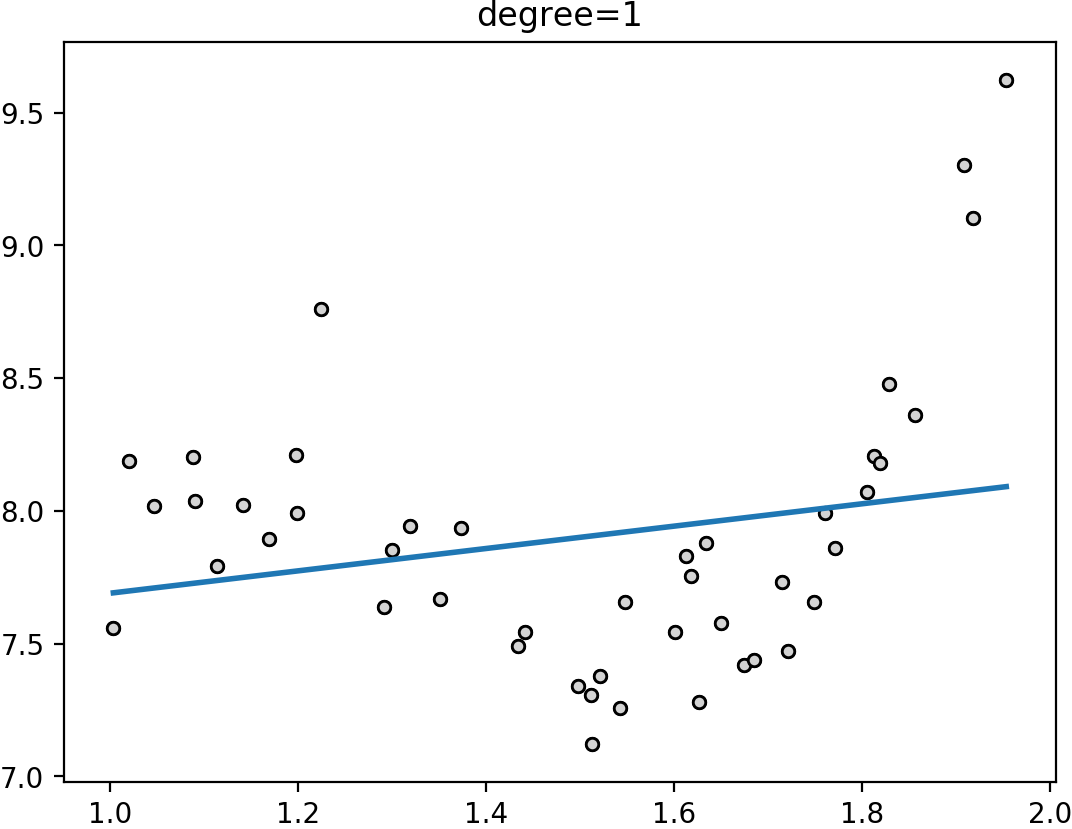
\includegraphics[width=\textwidth]{interp-pol-1.png}
    \end{figure}
\column{.33\textwidth}
\pause
    \begin{figure}
    \caption*{degree = 3 }
    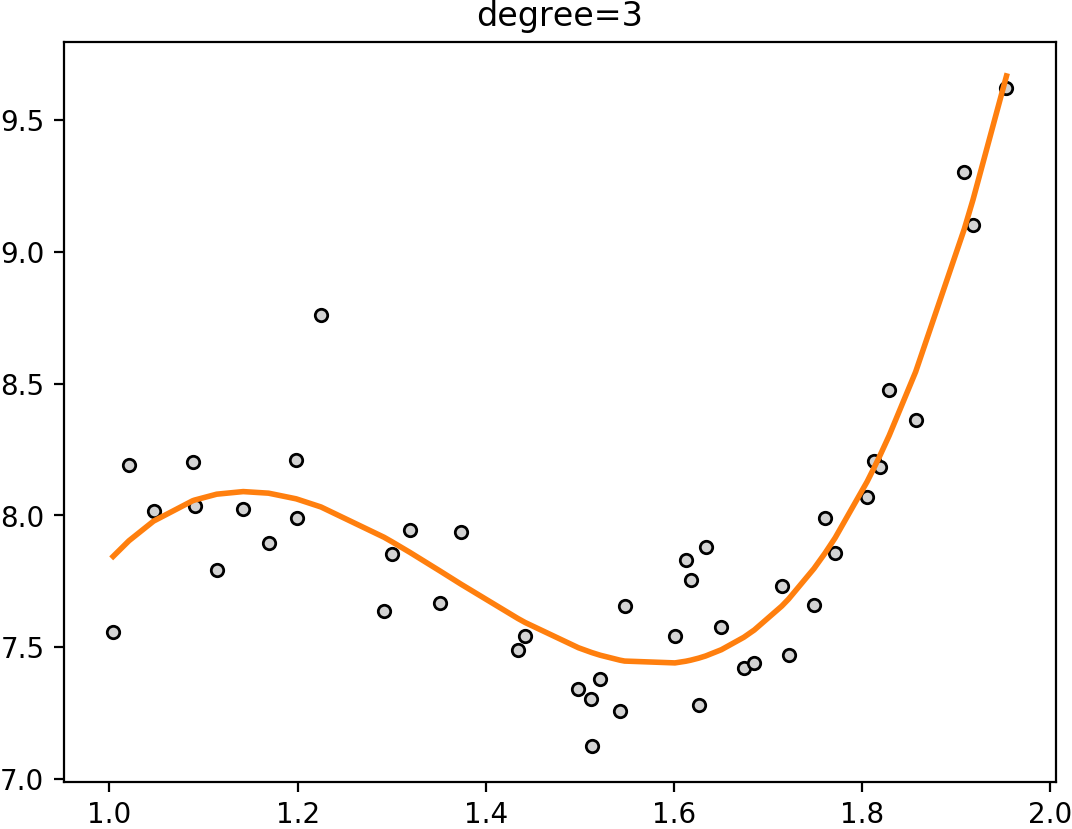
\includegraphics[width=\textwidth]{interp-pol-3.png}
    \end{figure}
\column{.33\textwidth}
\pause
    \begin{figure}
    \caption*{degree = 30 }
    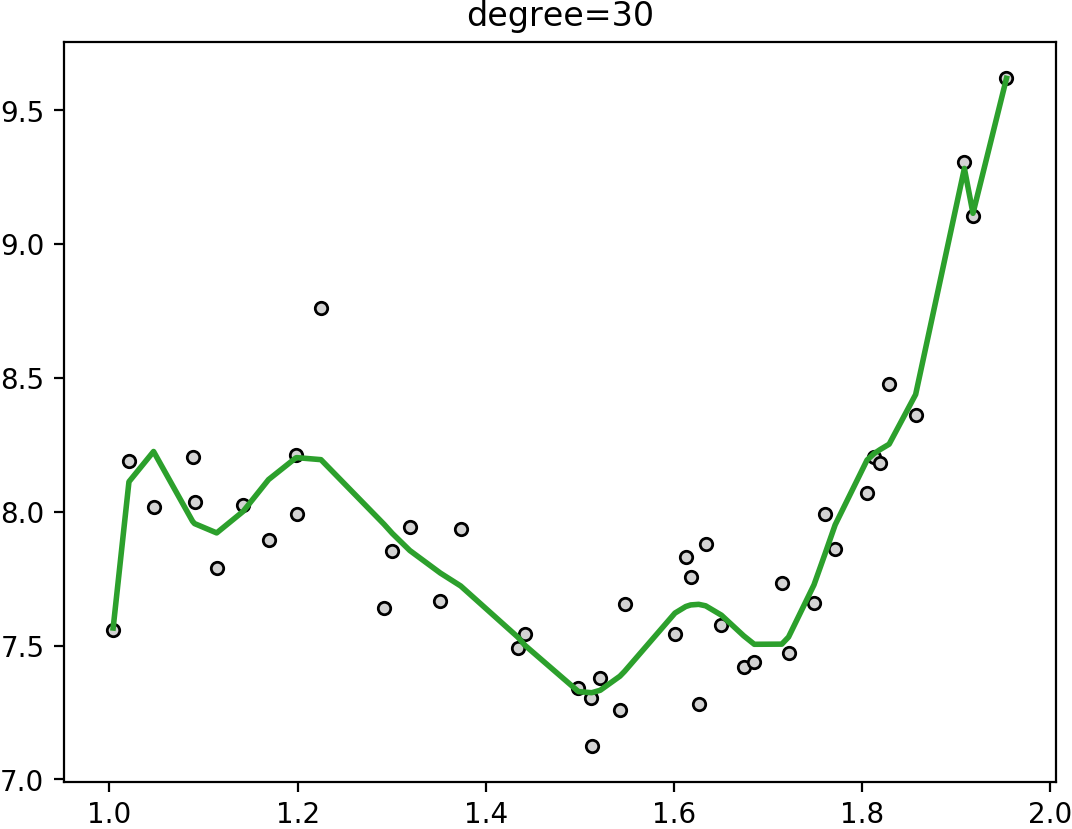
\includegraphics[width=\textwidth]{interp-pol-30.png}
    \end{figure}
 
\end{columns}
   
    \centering {
    \alert{What is the best model?}
    }
\end{frame}


%%%%%%%%%%%%%%%%%%%%
\begin{frame}{Train/Validation split}
\begin{block}{The idea}
Evaluate a score on a independent dataset
\end{block}
\pause
In our example we can randomly divide $(X,y)$ in two datasets:
\begin{itemize}
    \item The training dataset $X_{train},y_{train}$ used to fit the  model.
    \item The validation dataset $X_{val},y_{val}$ used to compute the score (e.g., correlation, mean-squared error)
\end{itemize}

    \begin{figure}
    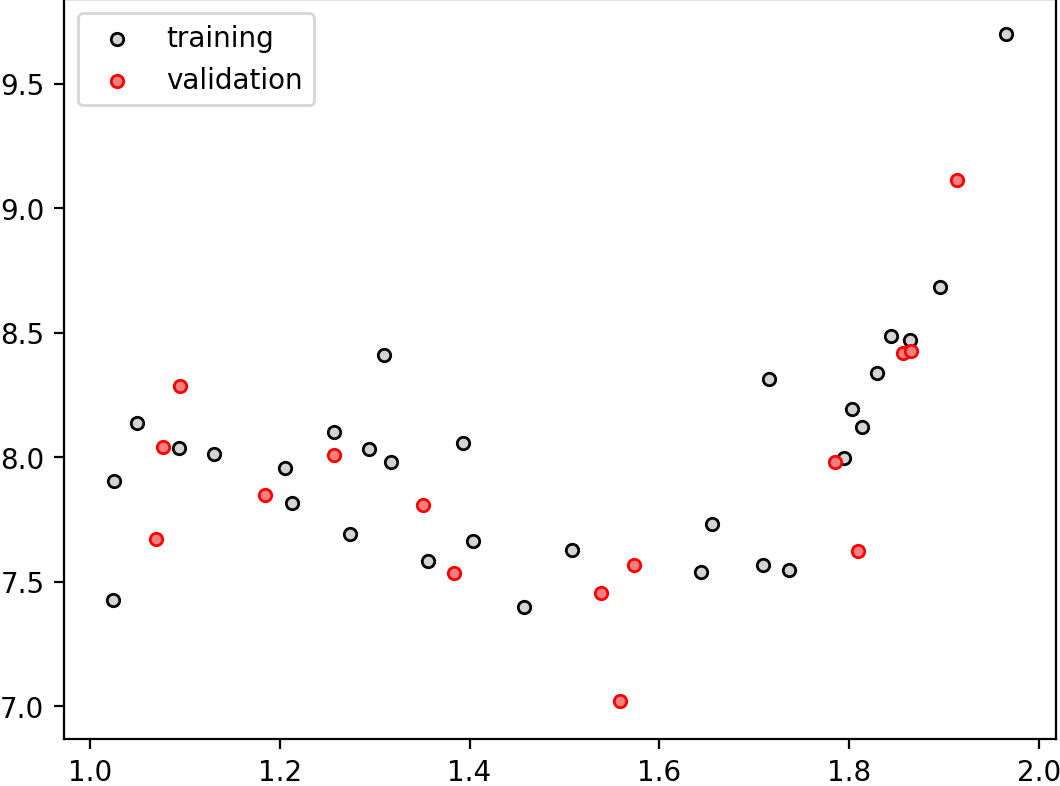
\includegraphics[width=.4\textwidth]{datasplit.png}
    \end{figure}

\end{frame}

%%%%%%%%%%%%%%%%%%%
\begin{frame}{Choice of the model}
\begin{columns}
\column{.5\textwidth}

    \begin{figure}
    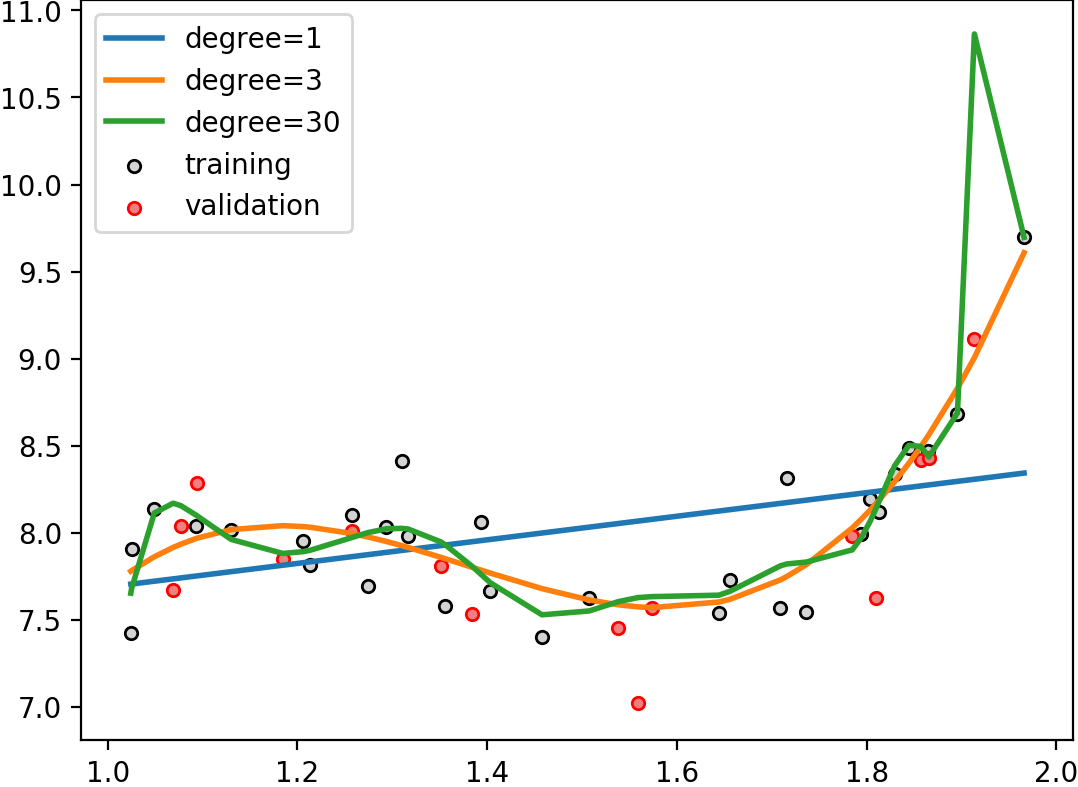
\includegraphics[width=\textwidth]{modelchoice.png}
    \end{figure}
\column{.5\textwidth}
Score: Mean Square Error (MSE)
\begin{table}
    \centering
    \begin{tabular}{c|c|c}
        Deg. & Train Score & Val. Score \\
        \hline
        1 & 0.17 & 0.23\\
        3 & 0.045 & 0.062\\
        30 & 0.035 & 0.27  \\
    \end{tabular}
    \end{table}
    %deg 1 ,score: val= 0.2283939842150192  , train= 0.167306864804612  , cv= 0.2768505679342689
%deg 3 ,score: val= 0.062492089527889656  , train= 0.04486320473714161  , cv= 0.05378120725339085
%deg 30 ,score: val= 0.27582336720042394  , train= 0.03473760406327127  , cv= 105306.65534552556
\end{columns}
\pause
   \begin{figure}
    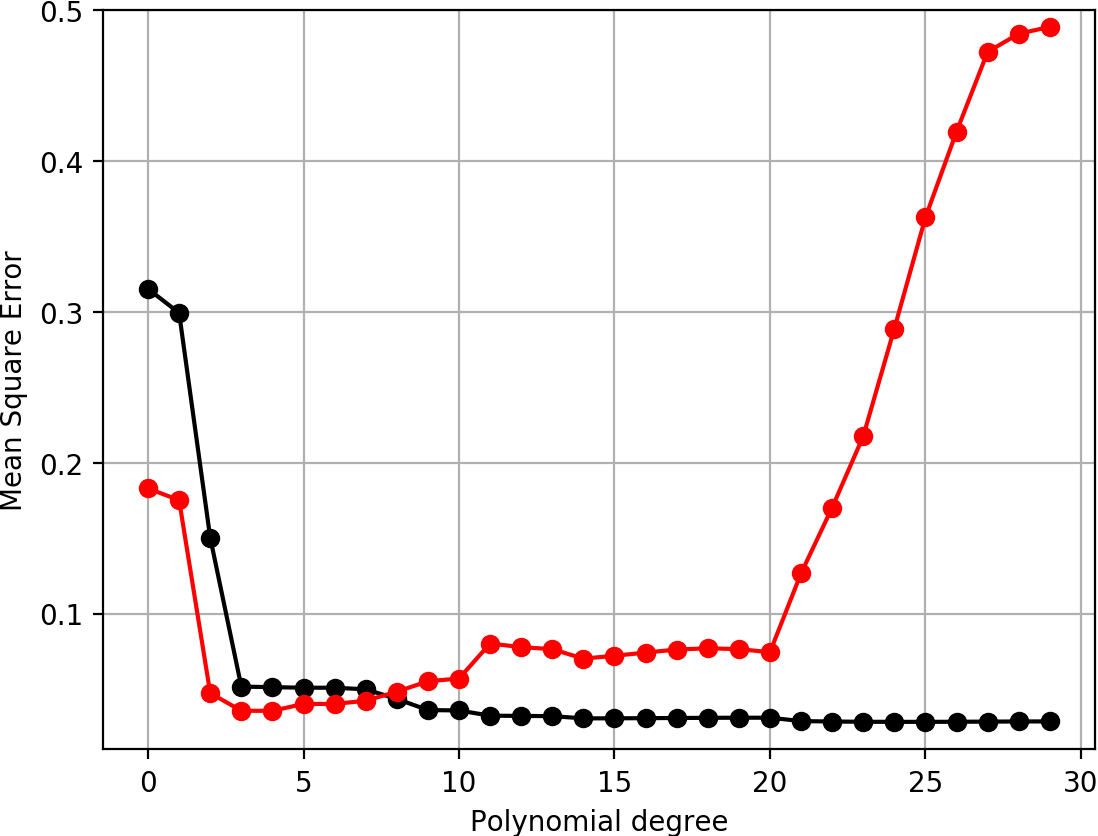
\includegraphics[width=.45\textwidth]{RMSE-deg-2scores.png}
    \end{figure}

\end{frame}

%%%%%%%%%%%%%%%%%%%%
\begin{frame}{Choice of the model}
\begin{block}{Polynomial regression}
$y=\theta_0 + \theta_1 x + \theta_2 x^2 + \cdots + \theta_d x^d = \sum_{i=0}^d \theta_i X^i$
\end{block}
\begin{columns}
\column{.33\textwidth}
    \begin{figure}
    \caption*{degree = 1 (linear)}
    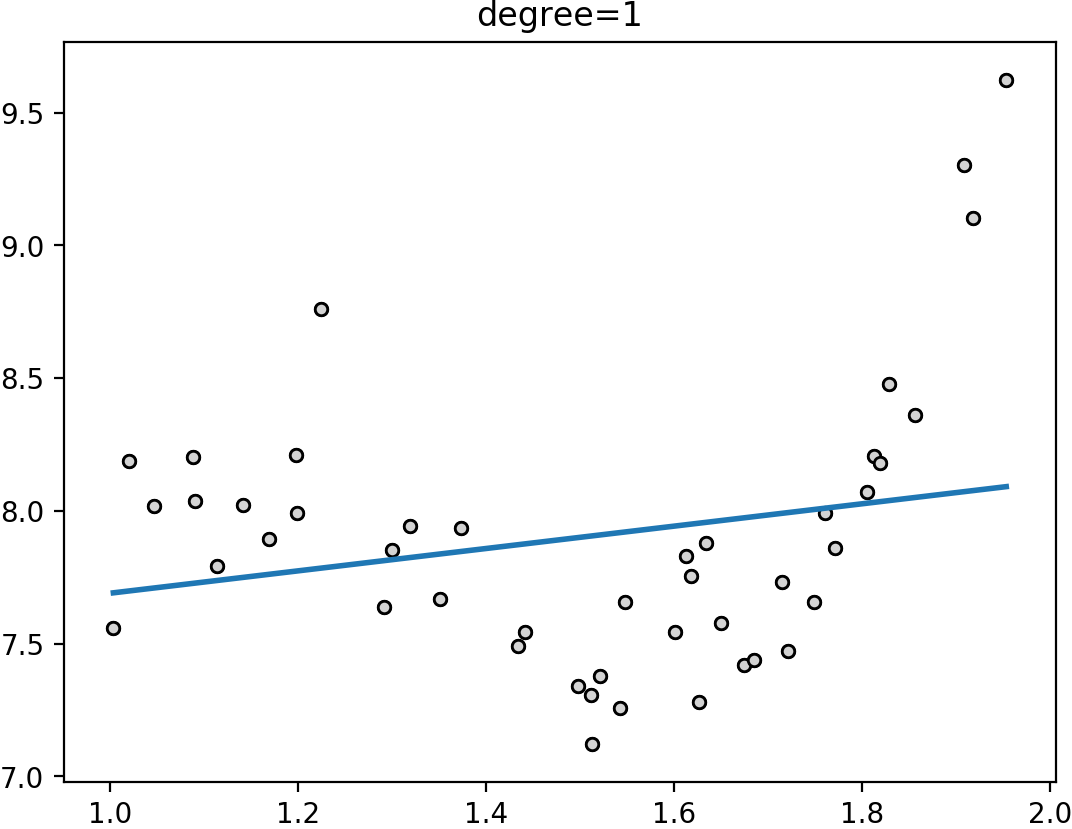
\includegraphics[width=\textwidth]{interp-pol-1.png}\\
        underfitting

    \end{figure}
\column{.33\textwidth}
    \begin{figure}
    \caption*{degree = 3 }
    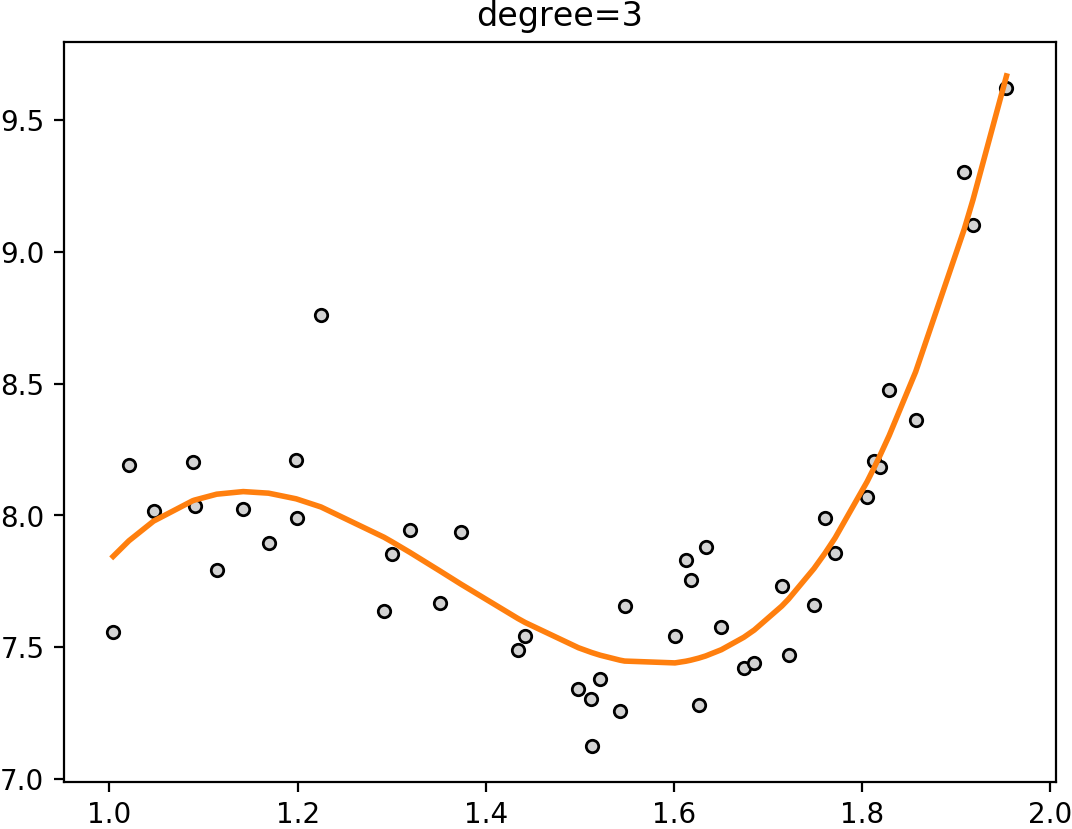
\includegraphics[width=\textwidth]{interp-pol-3.png}\\
        good fit

    \end{figure}
\column{.33\textwidth}
    \begin{figure}
    \caption*{degree = 30 }
    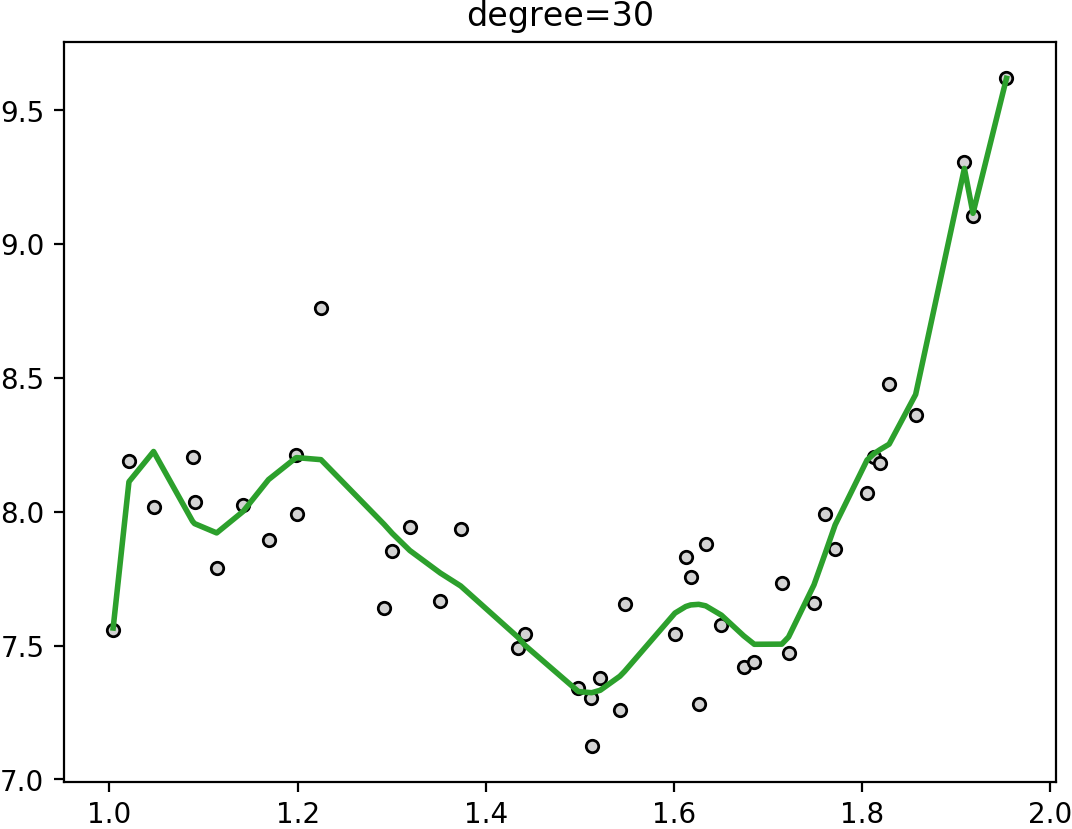
\includegraphics[width=\textwidth]{interp-pol-30.png}\\
        overfitting

    \end{figure}
 
\end{columns}

\end{frame}


%%%%%%%%%%%%%%%%%%%%
\begin{frame}{Train/Validation split}
     \begin{block}{Drawbacks}
\begin{itemize}
    \item drastically reduce the number of samples which can be used for learning the model
    \item Results  can depend on a particular random choice for the pair of (train, validation) sets.
\end{itemize}
\end{block}

\end{frame}
%%%%%%%%%%%%%%%%%%
\begin{frame}{More Robust: cross validation}
    \begin{block}{The idea}
    \begin{itemize}
\item Dividing the data in n folds, 
\item Learning n model (each time with a different training set),
\item Compute the mean score over n validation set.
\end{itemize}
\end{block}
   \begin{figure}
    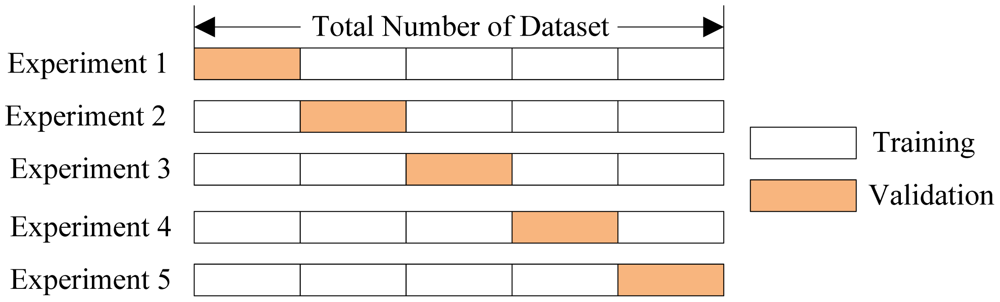
\includegraphics[width=\textwidth]{cv.png}
    \end{figure}

\end{frame}

%%%%%%%%%%%%%%%%%%%%
\begin{frame}{Cross-Validation}
\begin{columns}

\column{.3\textwidth}
\begin{table}
\footnotesize
    \centering
    \begin{tabular}{|c|c|}
    \hline
{\bf Fold} & {\bf MSE} \\
\hline
1 & 0.052 \\
2 & 0.043 \\
3 & 0.137 \\
4 & 0.025 \\
5 & 0.048 \\
6 & 0.144 \\
7 & 0.011 \\
8 & 0.025 \\
9 & 0.010 \\
10 & 0.028 \\
\hline
{\bf Mean} & {\bf 0.05} \\
        \hline


    \end{tabular}
    \end{table}
    
    \column{.7\textwidth}
   \begin{figure}
    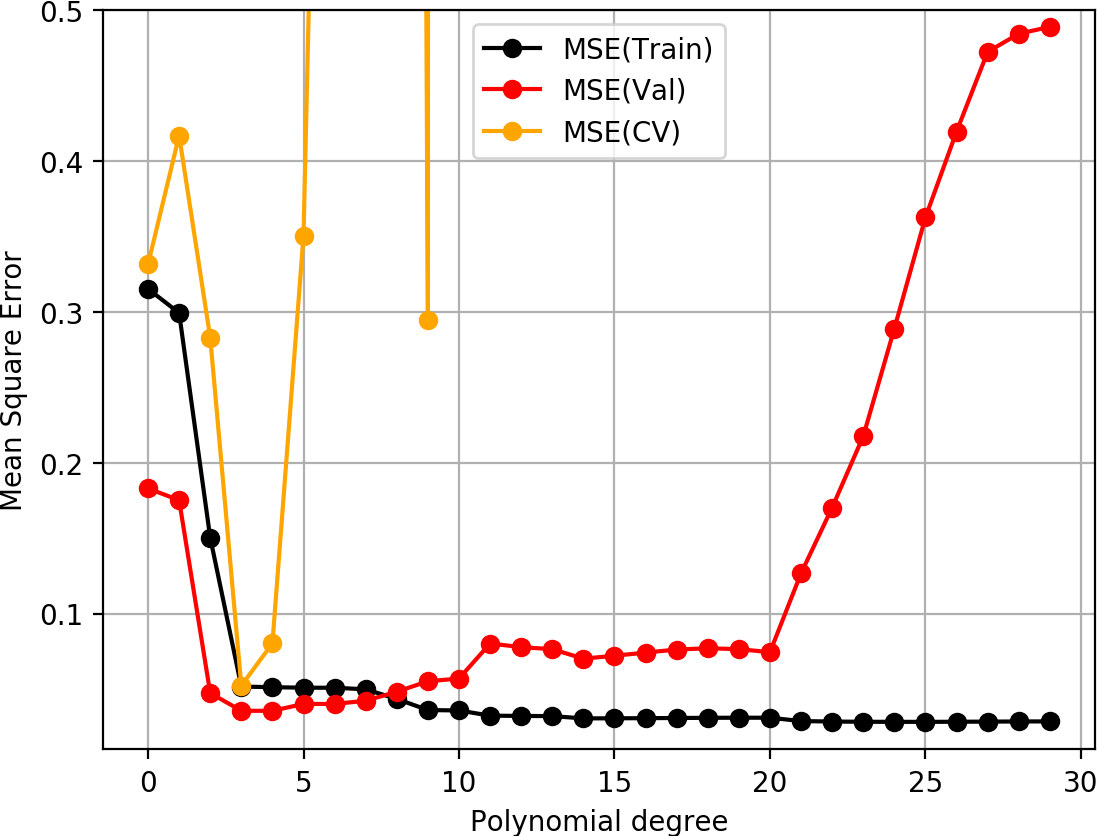
\includegraphics[width=\textwidth]{RMSE-deg-3scores.png}
    \end{figure}

\end{columns}

\end{frame}
%%%%%%%%%%%%%%%%
\begin{frame}{Wrapping up}
\begin{enumerate}[<+->]
    \item When applying machine learning techniques there are \alert{hyperparameters} to be determined (e.g., degree of the polynomial in polynomial regression).
    \item These \alert{hyperparameters}  can be determined by splitting the data into training/validation or by cross-validation.
    \item But then... the validation set was used to determine the best machine learning process
    \item To evaluate independanly the performance of our model, we should compute the score on a \alert{third independant dataset: The test dataset}.
    
\end{enumerate}
\end{frame}

\section{Case of auto-correlated data}

%%%%%%%%%%%%%%%%
\begin{frame}[fragile]{Random split}

\begin{itemize}[<+->]
\item A standard way to select the validation is to split randomly the dataset at a given proportion.\\
\textit{If 15\% of the point is in the validation set, each sample ${\bf x}_i$ has a probability of 15\% to be in the validation set}
\item It can be done using the sklearn python library
\begin{lstlisting}[language=Python]
from sklearn.model_selection import train_test_split

X_train, X_test, y_train, y_test = 
    train_test_split(X, y, test_size=0.15)
\end{lstlisting}
\item {\large \textcolor{red}{WARNING!}} It can lead to problems with auto-correlated data (e.g. pixels of an image, time series).\\
\alert {More exactly}: it leads to problem if the residual between the target and the model prediction (a.k.a. model error) is auto-correlated.
\end{itemize}
\end{frame}

%%%%%%%%%%%%%%%%
\begin{frame}{Illustration}
\begin{columns}

 \column{.3\textwidth}
   \begin{figure}
    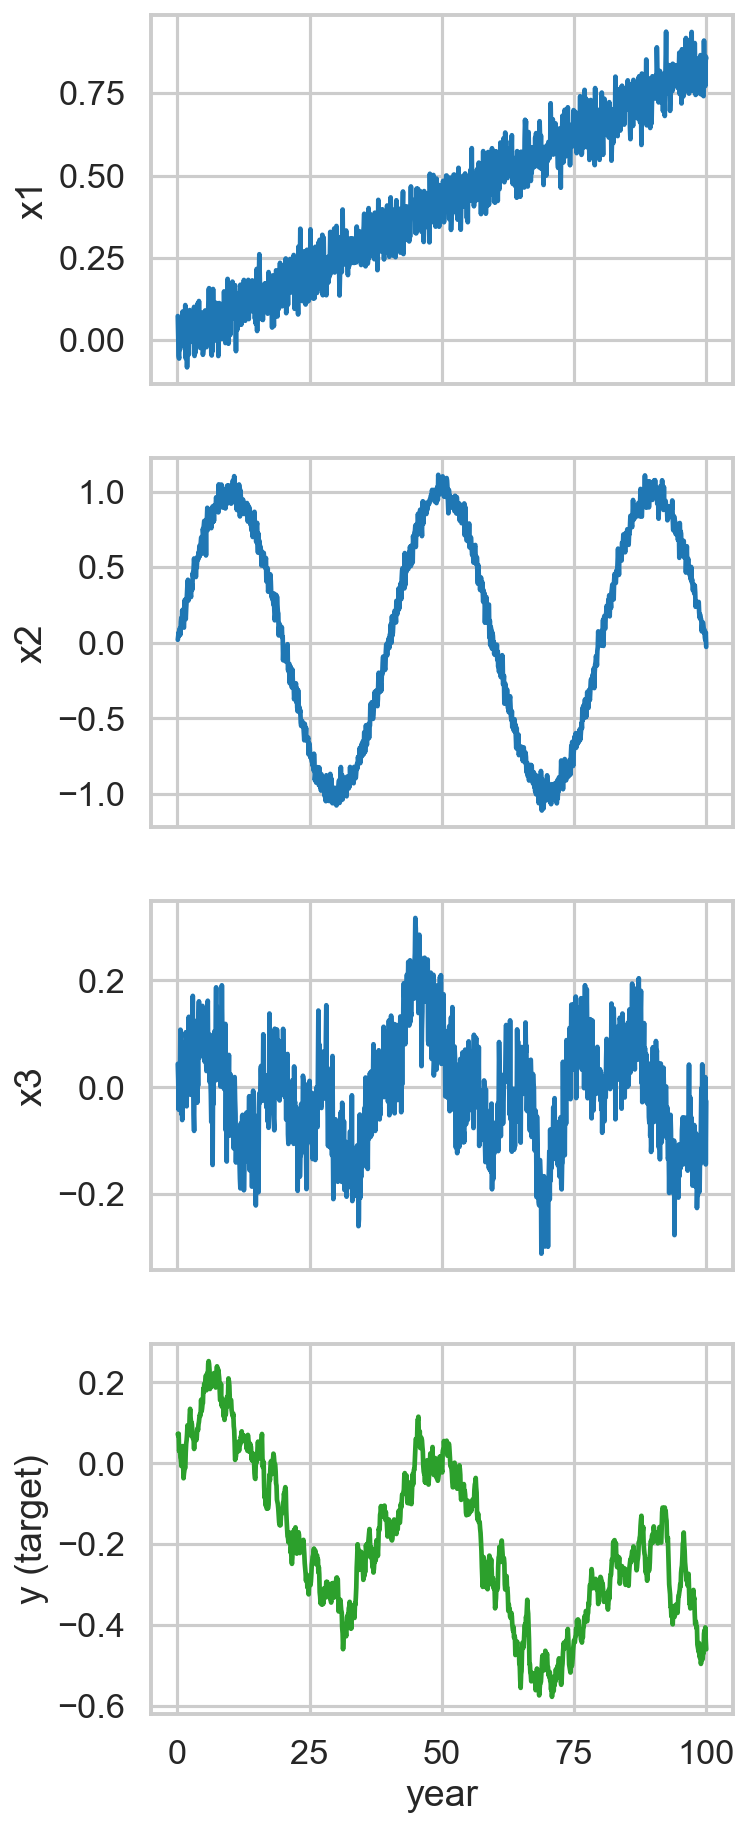
\includegraphics[width=\textwidth]{presentation/course-2/figs/leak_data.png}
    \end{figure}
    
    
\column{.7\textwidth}
\alert{Objective:} predict the target $y$ from the three features $x_1, x_2$ and $x_3$.\\
\vspace{2em}
Note: this is an artificial problem that have been created for the illustration. The true model is known:\\
$ y = -\frac{1}{2} x_1 + \frac{1}{5} x_2 +\frac{1}{5} x_3$

\pause
\begin{block}{Model and metric}
We will use a polynomial regression and chose the polynomial degree of the best nodel (in term of mean square error) from a validation set
\end{block}

\end{columns}

\end{frame}

%%%%%%%%%%%%%%%%
\begin{frame}{Result with random split}
\begin{columns}
\column{.5\textwidth}
   \begin{figure}
    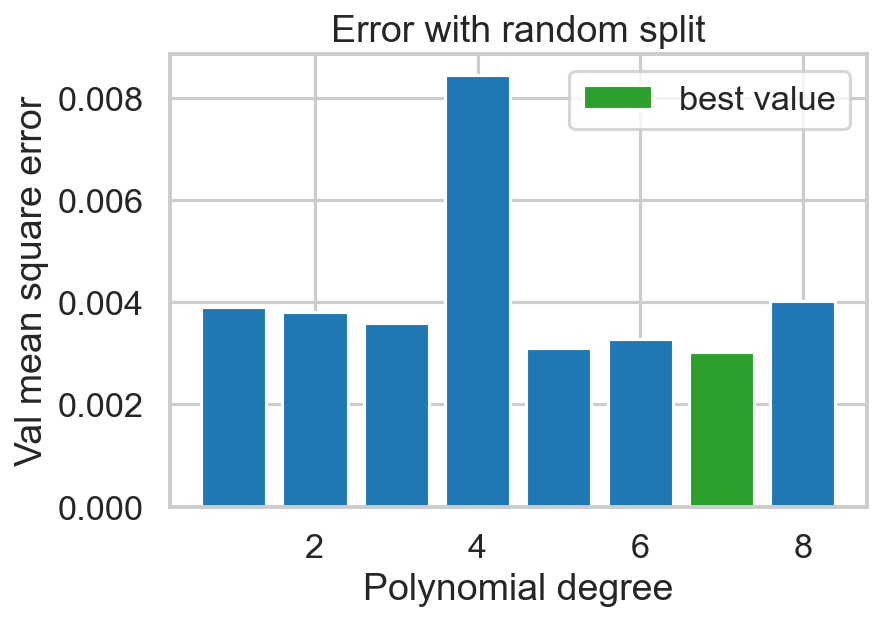
\includegraphics[width=.9\textwidth]{presentation/course-2/figs/leak_bar_random.png}
    \end{figure}
    
\column{.5\textwidth}
   \begin{figure}
    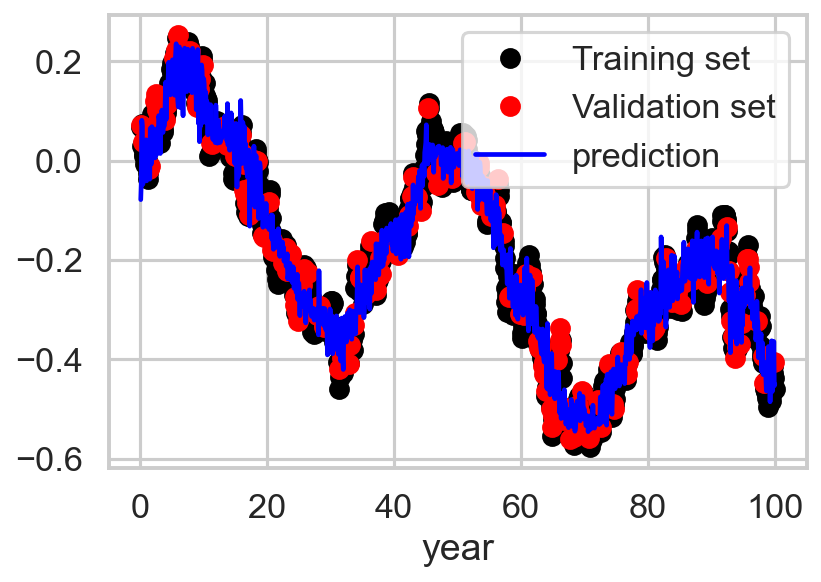
\includegraphics[width=.9\textwidth]{presentation/course-2/figs/leak_ts_random.png}
    \end{figure}
\end{columns}

   \begin{figure}
   \centering
   Can the model determine ($d=7$) generalize to new data? (year > 100)\\
   \pause
    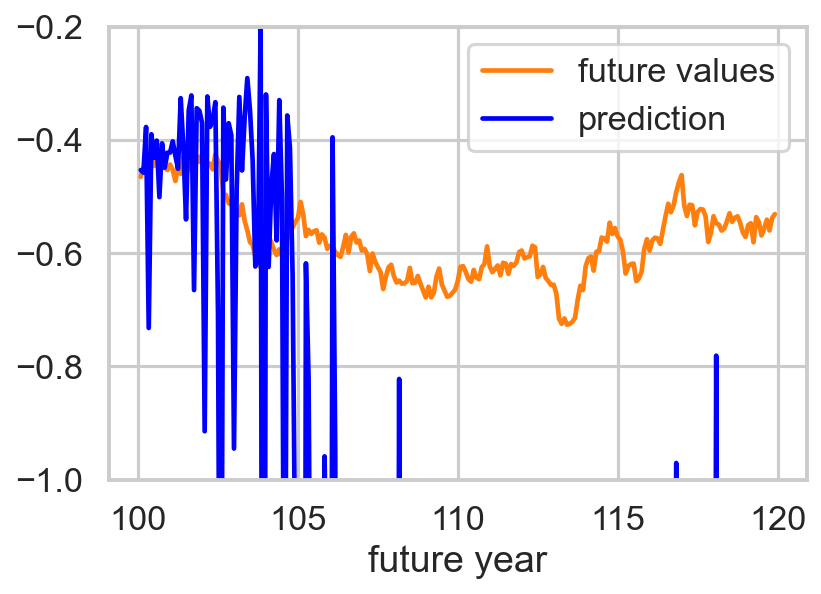
\includegraphics[width=.5\textwidth]{presentation/course-2/figs/leak_test_random.png}
    \end{figure}
\end{frame}


%%%%%%%%%%%%%%%%
\begin{frame}{Result with random split}

%%%%%%%%%%%%%%%%
\begin{frame}{Result with random split}
\begin{columns}
\column{.5\textwidth}
   \begin{figure}
    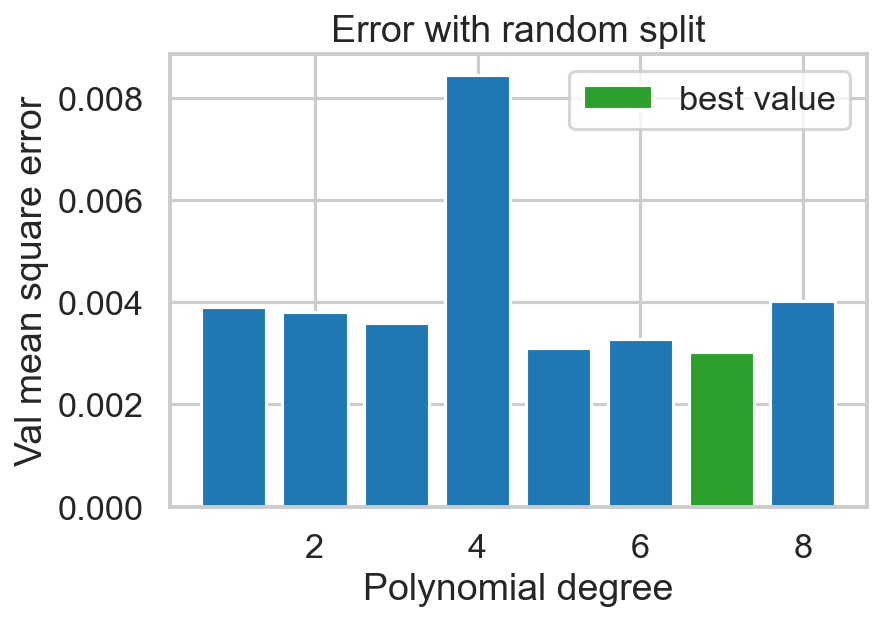
\includegraphics[width=.9\textwidth]{presentation/course-2/figs/leak_bar_random.png}
    \end{figure}
    
\column{.5\textwidth}
   \begin{figure}
    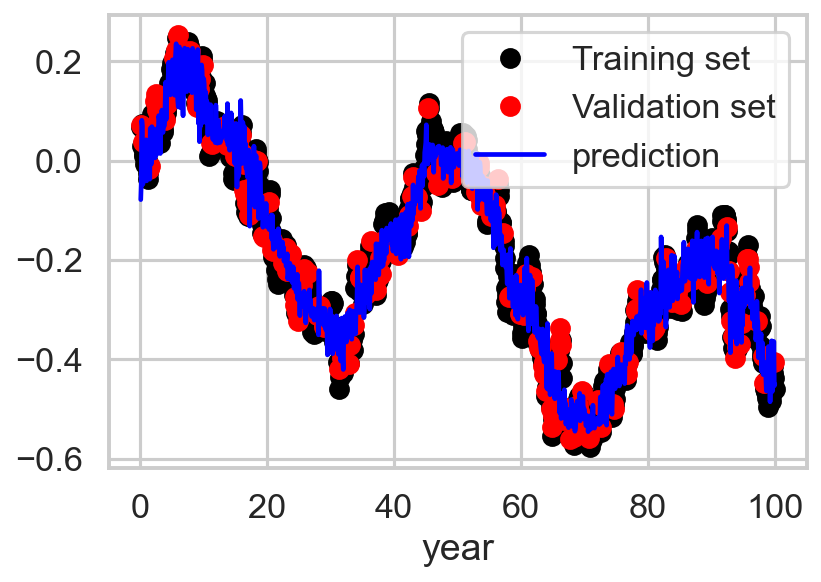
\includegraphics[width=.9\textwidth]{presentation/course-2/figs/leak_ts_random.png}
    \end{figure}
\end{columns}

   \begin{figure}
   \centering
   Can the model determine ($d=7$) generalize to new data? (year > 100)\\
   \pause
    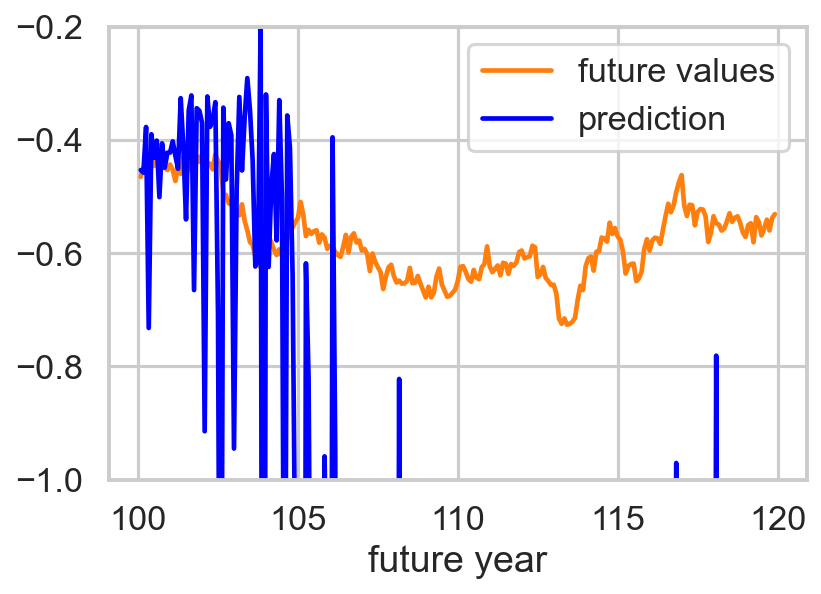
\includegraphics[width=.5\textwidth]{presentation/course-2/figs/leak_test_random.png}
    \end{figure}
\end{frame}


\section{Steps of a machine learning process}

%%%%%%%%%%%%%%%%
\begin{frame}{Steps}
    \begin{figure}
        \centering
     \tikzstyle{block} = [rectangle, draw, fill=blue!20, text width=7em, text centered, rounded corners, minimum height=4em]
     \tikzstyle{line} = [draw, ->]
    \tikzstyle{back} = [draw, ->, very thick, red]
     
     \begin{tikzpicture}[auto, node distance=1cm and 2cm]
     \node[block] (collect) {Collect data} ;
     
     \pause
     \node [block, below= of collect] (feature) {Preprocess /clean data\\\footnotesize{\textit{feature extractions}}};
     \path [line] (collect)--(feature);

     \pause
     \node  [block, right= of collect] (tune) {Design model};
     
     \pause
     \node  [block, right= of feature] (train) {Train model};
     \path  [line] (feature)-- node[above]{train} (train);
     \path  [line] (tune)-- (train);
     
     \pause
     \node  [block, below= of train] (evaluate) {Evaluate model};
     \path  [line] (train)--(evaluate);
     \path  [line]  (feature) --  node[above,sloped]{(cross-)valid}(evaluate);

     \pause
     \path  [back]  (evaluate) edge[bend right=80] (tune);
     \path  [back]  (evaluate) edge[bend left] (feature);
     \path  [back]  (evaluate) edge[bend right] (collect);
     
     \pause
     \node  [block, fill=red!20, left=of evaluate]  (release) {Release model};
     \path  [line]  (evaluate)--(release);
     \path  [line]  (feature) -- node[above,sloped]{test} (release);

    

     \end{tikzpicture}
    \end{figure}
\end{frame}

%%%%%%%%%%%%%%%%%%%%%%%%%%%%%%%%%%%%%%%%%%
\begin{frame}{In summary}
    From one dataset, 3 sub-datasets have to be extracted:
    \begin{itemize}
        \item A training dataset
        \item A validation dataset
    \end{itemize}
    Can be done iteratively in a cross-validation procedure.\\
    \alert {Some parameters of the model (e.g. polynomial order in a polynomial regression) were determined from the validation dataset.}
    \begin{itemize}
        \item A test dataset (independent from the two other) to estimate the final performance of the model.
    \end{itemize}
\end{frame}




\end{document}